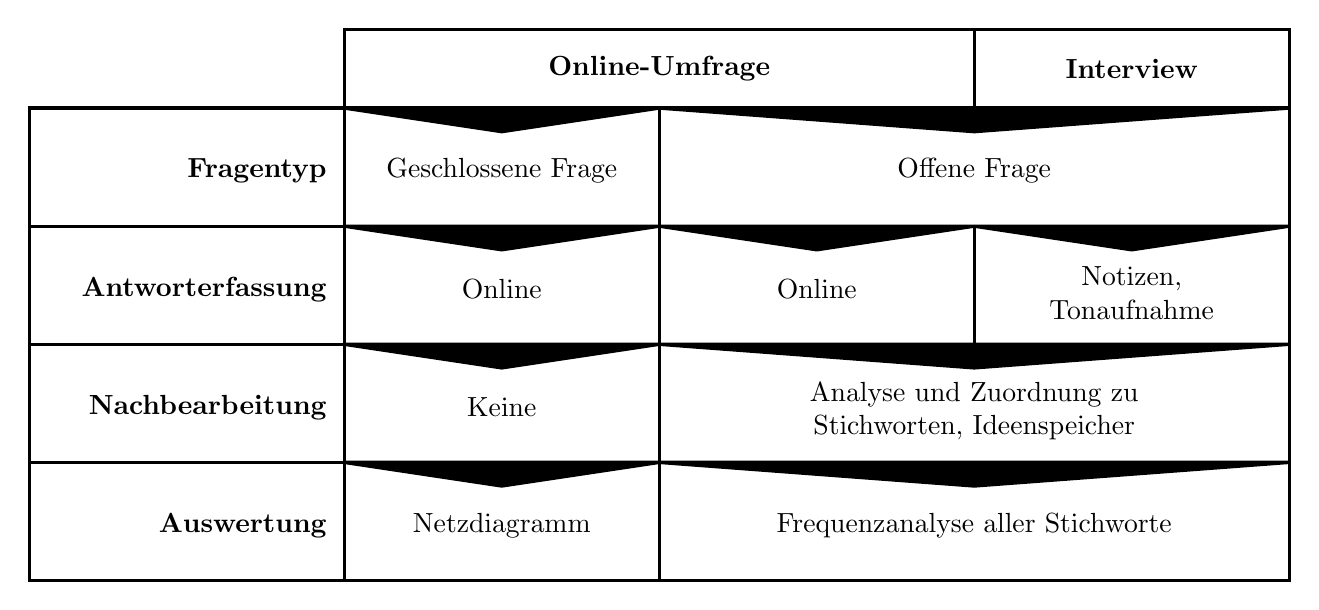
\begin{tikzpicture}

%% - Draw helping gridlines
%% - --------------------------------------

%\draw[step=2cm,gray,very thin] (0,0) grid (16,9);

%% - Draw table
%% - --------------------------------------

%\draw[black,very thick] (0,0) rectangle (16,2);
%\draw[black,very thick] (0,2) rectangle (16,4);
%\draw[black,very thick] (0,4) rectangle (16,6);
%\draw[black,very thick] (0,6) rectangle (16,8);
%\draw[black,very thick] (4,0) rectangle (8,8);
%\draw[black,very thick] (4,8) rectangle (16,9);
%\draw[black,very thick] (12,8) -- (12,9);
%\draw[black,very thick] (12,4) -- (12,6);

\draw[black,very thick] (0,0) rectangle (16,1.5);
\draw[black,very thick] (0,1.5) rectangle (16,3);
\draw[black,very thick] (0,3) rectangle (16,4.5);
\draw[black,very thick] (0,4.5) rectangle (16,6);
\draw[black,very thick] (4,0) rectangle (8,6);
\draw[black,very thick] (4,6) rectangle (16,7);
\draw[black,very thick] (12,6) -- (12,7);
\draw[black,very thick] (12,3) -- (12,4.5);

%% - Draw filled arrows
%% - --------------------------------------
%% - geschlossene Frage
%% - --------------------------------------
\filldraw[color=black,fill=black,very thick] (4,6) -- (8,6) -- (6,5.7) -- cycle;
%% - geschlossene Frage Online
%% - --------------------------------------
\filldraw[color=black,fill=black,very thick] (4,4.5) -- (8,4.5) -- (6,4.2) -- cycle;
%% - geschlossene Frage Keine
%% - --------------------------------------
\filldraw[color=black,fill=black,very thick] (4,3) -- (8,3) -- (6,2.7) -- cycle;
%% - geschlossene Frage Netzdiagramm
%% - --------------------------------------
\filldraw[color=black,fill=black,very thick] (4,1.5) -- (8,1.5) -- (6,1.2) -- cycle;
%% - Offene Frage
%% - --------------------------------------
\filldraw[color=black,fill=black,very thick] (8,6) -- (16,6) -- (12,5.7) -- cycle;
%% - Analyse & Zuordnung zu Stichworten
%% - --------------------------------------
\filldraw[color=black,fill=black,very thick] (8,3) -- (16,3) -- (12,2.7) -- cycle;
%% - Frequenzanalyse aller Stichworte
%% - --------------------------------------
\filldraw[color=black,fill=black,very thick] (8,1.5) -- (16,1.5) -- (12,1.2) -- cycle;
%% - Online
%% - --------------------------------------
\filldraw[color=black,fill=black,very thick] (8,4.5) -- (12,4.5) -- (10,4.2) -- cycle;
%% - Notizen, Tonaufnahme
%% - --------------------------------------
\filldraw[color=black,fill=black,very thick] (12,4.5) -- (16,4.5) -- (14,4.2) -- cycle;

%% - Draw Text
%% - --------------------------------------
\node[draw,scale=1,shape=rectangle,draw=none,anchor=east,font=\bf] at (3.9,5.2) {Fragentyp};
\node[draw,scale=1,shape=rectangle,draw=none,anchor=east,font=\bf] at (3.9,3.7) {Antworterfassung};
\node[draw,scale=1,shape=rectangle,draw=none,anchor=east,font=\bf] at (3.9,2.2) {Nachbearbeitung};
\node[draw,scale=1,shape=rectangle,draw=none,anchor=east,font=\bf] at (3.9,0.7) {Auswertung};

\node[draw,scale=1,shape=rectangle,draw=none] at (6,5.2) {Geschlossene Frage};
\node[draw,scale=1,shape=rectangle,draw=none] at (6,3.7) {Online};
\node[draw,scale=1,shape=rectangle,draw=none] at (6,2.2) {Keine};
\node[draw,scale=1,shape=rectangle,draw=none] at (6,0.7) {Netzdiagramm};

\node[draw,scale=1,shape=rectangle,draw=none] at (12,5.2) {Offene Frage};
\node[draw,scale=1,shape=rectangle,draw=none,text width=7cm,align=center] at (12,2.15) {Analyse und Zuordnung zu Stichworten, Ideenspeicher};
\node[draw,scale=1,shape=rectangle,draw=none] at (12,0.7) {Frequenzanalyse aller Stichworte};

\node[draw,scale=1,shape=rectangle,draw=none] at (10,3.7) {Online};
\node[draw,scale=1,shape=rectangle,draw=none,text width=3cm,align=center] at (14,3.65) {Notizen, Tonaufnahme};

\node[draw,scale=1,shape=rectangle,draw=none,font=\bf] at (8,6.5) {Online-Umfrage};
\node[draw,scale=1,shape=rectangle,draw=none,font=\bf] at (14,6.5) {Interview};

\end{tikzpicture}
